\documentclass[12pt]{paper}
\usepackage[margin=1in]{geometry}
\usepackage{float}
\usepackage{natbib}
\bibliographystyle{apsr}
\usepackage{graphicx}
\graphicspath{ {../fig/} }
\usepackage{setspace}
\usepackage[super]{nth}
\usepackage{booktabs}
\usepackage{makecell}
\usepackage{amsmath}
\usepackage{dcolumn}
%\usepackage{authblk}
\usepackage{hyperref}
\usepackage{wrapfig}
\usepackage{amsmath}
\usepackage{adjustbox}
\usepackage{hanging}
%\usepackage{etoolbox}
%\AtBeginEnvironment{quote}{\singlespacing\small}

\newlength{\cslhangindent}
\setlength{\cslhangindent}{1.5em}
\newenvironment{cslreferences}%
{\setlength{\parindent}{0pt}%
	\everypar{\setlength{\hangindent}{\cslhangindent}}\ignorespaces}%
{\par}

\title{Untitled White Nationalism Project}
\author{Sarah R. Warren}
\date{}

\begin{document}
\maketitle
%\thispagestyle{empty}
%\clearpage
%\setstretch{1}

\doublespacing
\section*{Introduction}
Over the past five years, mainstream American politics has seen a distinct rise in white-nationalist and neo-Nazi activity. From the Unite the Right rally in Charlottesville, Virginia in 2017 to the White Civil Rights Rally in Washington, D.C. in 2018, these events purported to solve a collective action problem. These events sparked renewed concern and interest in white nationalism, which is notable because many Americans believe the United States has virtually eradicated racism (Krysan and Moberg 2016). In a public that has operated under the illusion of postracialism for so long, these attacks and the seemingly-overnight popularity of white nationalism was particularly surprising. These events raise several important questions for scholars of political violence. In particular, who are the white nationalists of the 21st Century? How are they mobilizing and what set of ideas are they mobilizing around? In the digital age, how are they leveraging the Internet to their advantage? The answers to these questions not only inform us about white nationalists, but help us understand them in the context of the digital age.

To address these questions about white nationalists in the mass public, we need an environment in which scientists can observe their behavior, thoughts, and feelings, but where they do not know they are being directly observed. This is critical, because observation is likely to alter speech in the case of socially undesirable ideas (Nederhof 1985). The small body of work on white nationalists who are not public figures focuses on exclusively on their online communities or the spreading of “digital hate” on websites like Reddit and Twitter (Daniels 2018; Berlet and Mason 2019), but these platforms have strict content restrictions. Users expressing white supremacy are frequently banned and alt-right subreddits are frequently deleted. While this is normatively desirable insofar as it stifles hate-groups' ability to proselytize, it inhibits our understanding of \textit{what} these communities are saying and \textit{how} they are saying it.

To circumvent this kind of selection bias without violating these platforms’ Terms of Service by retaining deleted content, this paper presents a novel dataset of posts from StormFront.org, the largest white nationalist forum on the internet. This paper presents the dataset, which is publicly available for use and replication,  and endeavors to address the questions above by offering one of the first in-depth examinations of non-elite white nationalist ideology and rhetoric (for other examples, see: Thompson 2001; Wojcieszak 2010; and Hartzell 2020).  

To preview my results, I find that past work has largely failed to appropriately understand the \textit{context} of StormFront.org before analyzing texts therein (but see: Hartzell 2020). When we understand the context of the forum as a public-facing recruitment mechanism for disaffective whites, the relative lack of racial epithets and hate speech begins to make sense. However, hidden groups on the forum for members only belie much darker sentiments that are not accessible to watchdogs, webscraping, or the general public.

The rest of this paper proceeds as follows. Section I introduces the data-generating process and data collection procedure. It introduces the context in which the forum posts were produces and what they do and do not contain, providing context for how we should interpret their content. Section II considers the contents of forum posts, using Structural Topic Modeling (STM) to describe the topics discussed within and across threads. It further considers the affect of forum posts, using sentiment analysis to describe the sentiments associated with topics within and across subforums. Section III concludes with a discussion of these descriptive results and thoughts for future work.

\section{Section I: StormFront.org}
There is a paucity of scholarly work concerning StormFront.org. Often, it makes use of a small sample of interviews (De Koster and Houtman 2008) or rhetorical analysis of a handful of posts (Bowman-Grieve 2009; Hartzell 2020). Scholarship which does make use of large corpi of texts from the forum often uses it to \textit{categorize} behavior - for example, exploring the prevalence of hate speech (Gibert et al.
2018) or posting patterns in the Opposing Views Forum (Bright et al. 2022), which is open to guests and even translated into Spanish, Portuguese, and French for international visitors. This article, by contrast, not only introduces a novel dataset of StromFront.org forum posts, but offers the first in-depth contextualization of StormFront.org.

StormFront.org is a typical virtual community, characterized by in-group norms, strong enforcement of these norms by moderators, and a specific set of shared interests and values (De Koster and Houtman 2008; Bowman-Grieve 2009). It is the largest white nationalist website on the internet, boasting over 60,000 unique viewers a day. It was created in 1995 by former Ku Klux Klan (KKK) leader Don Black and has been called the “first major hate site on the Internet.” In 2001, StormFront transitioned from a simple webpage to an interactive message board. By 2005, that forum had grown to over 40,000 registered members and Stormfront was independently ranked within the top 1 percent of all websites in terms of activity (CITE). StormFront has since grown to hundreds of thousands of members and regularly tracks tens of thousands of unregistered guest browsers each day.

StromFront.org, which boasts that ``Every month is white history month," is dedicated to fostering discussion and community among white nationalists around the world. White nationalism is a derivative of white supremacy which advocates for racial seperatism, a white ethnostate, and the preservation of white racial hegemony (\textit{Southern Poverty Law Center}). White nationalists attempt to distinguish themselves from white supremacists, arguing that they are not fueled by hatred or bigotry, but rather a desire to protect and preserve white identity in a culture of white erasure. Many others (Meddaugh and Kay 2009; Hartzell 2020) have noted that StormFront users only employ the dispassionate, academic rhetoric of ``reasonable racism" in an attempt to legitimize their viewpoints. Indeed, the posting guidelines on StormFront.org ban the use of racial epithets and profanity, warning, ``Before you post anything, remember that words have consequences, both for you and others. This is true even if they're posted pseudonymously on a discussion board," (https://www.stormfront.org/forum/t4359/). Given this, there is a surprising lack of hate speech on StormFront.org (Gilbert et al. 2018).

Bearing in mind that StormFront.org can be viewed by anyone and even has forums open to visitors where they can ask questions and share opposing viewpoints, this polished rhetoric makes sense. StormFront.org appears to be not only a virtual community for white nationalists, but a recruitment tool for disaffected whites (De Koster and Houtman 2008; Bowman-Grieve 2009). To get to the real extremism, one has see what only members can, what's not accessible to the general public.

A reality heretofore not discussed by scholars of online white nationalism is that a great deal of the activity on StormFront.org is hidden behind a membership wall. That is, it is unavailable to visitors without an account. If one joins the forum, one quickly sees that a great deal of activity occurs in ``Groups," which are private and separate from public-facing discussion boards. Many groups are run by site moderators and prominent users; access is invitation-only or, if you believe you should have access, you can submit references for gatekeepers to contact to verify your value to ``the cause." Members who are ``one post wonders" are rarely allowed into any groups, regardless of whether they are invitation-only or open to most users.

Users are encouraged to post and participate in forum culture, to keep threads and groups active, and to exchange contact information to create real-life communities. While past work has noted that StormFront.org functions as a virtual community for disaffected whites (Bowman-Grieve 2009; Meddaugh and Kay 2009; Hartzell 2020), the mechanisms by which community is stimulated have remained hidden. The private network of social groups, private messaging, and the funnel from StormFront.org to private forums and chatrooms by invitation only are hidden from mere visitors.

All users who join the forum are sent an automated greeting message from Don Black. A few days later, notable white nationalist and ``Farm Belt Fuhrer" Gerhard Lauck sends along links to websites where new members can purchase translated Nazi materials popularized during the Third Reich. These include children's books like \textit{The Poisonous Mushroom} by Julius Streicher, war criminal and the publisher of \textit{Der Stürmer}.\footnote{The full text of these messages can be found in Appendix A.} 

It is clear that there is a communal understanding that some topics and sentiments are expressed only behind the wall of membership, in the safety of private social groups. Indeed, only a cursory search of the private social groups yields access to much more extreme content than is found on the publicly accessible forum. For example, there is a private social group called ``The Brotherhood" for ``those willing to do whatever it takes to secure the existence of our people. A group we may require in the future..." There is a private group for males only, with numerous threads dedicated to foreskin restoration because white nationalists consider circumcision genital mutilation. There is also a private group for ``Stormfronters Younger than 18," where the most popular threads include minors posting their ages, their ancestry, and debating ``the homosexual question."

The existence of these private, member-only groups is important for our understanding of any data from StormFront.org. Users are at least somewhat cognizant that anything they say or write may be seen by the public or ``lurkers," those who read the forums without joining. We should, therefore, not expect completely \textit{candid} speech from the public-facing forums; instead, we should expect a polished version of what white nationalists \textit{want} the world to know about them, underscored by strict posting guidelines. Still, using these data to obtain speech absent the confines of social desirability bias is still appropriate. Speech may not be entirely \textit{candid}, due to strict posting guidelines, but we have no reason to suspect that an inability to use slurs will change the underlying sentiment expressed. The pseudonymous nature of the forum protects individual identities and allows for the sharing of genuine sentiment with limited ``real world" consequences. A similar approach was taken by Wu (2020) using the Economic Job Market Rumors Forum. The relatively niche nature of the forum, combined with the use of pseudonyms, lends credibility to the argument that users are more free to express their unaltered opinions in these contexts than on surveys and other information environments. Further, the forum is dedicated to white nationalist ideation. One could characterize the purpose of StormFront.org as the pseudo-anonymous sharing of socially undesirable opinions. The website has sub-forums dedicated to different topics such as revisionist history, culture, COVID-19, philosophy, politics, and white nationalist ideology, making it easier for users and researchers to obtain speech on specific topics.

The data I present here were scraped on September 7, 2021 and come from the three most popular public-facing threads (National Socialism, Positive White Nationalism, and Conservatism) on the Ideology and Philosophy subforum as of the day of scraping. There are a total of 5,423 unique posts, including the full text of the post, the username of the poster, the date and time it was posted, the forum to which it was posted, and the length of the post in characters.  Due to the private nature of social groups and messages, the data that I present here do not include any activity therein; they contain only data from the public-facing forums. 

\begin{figure} \centering
	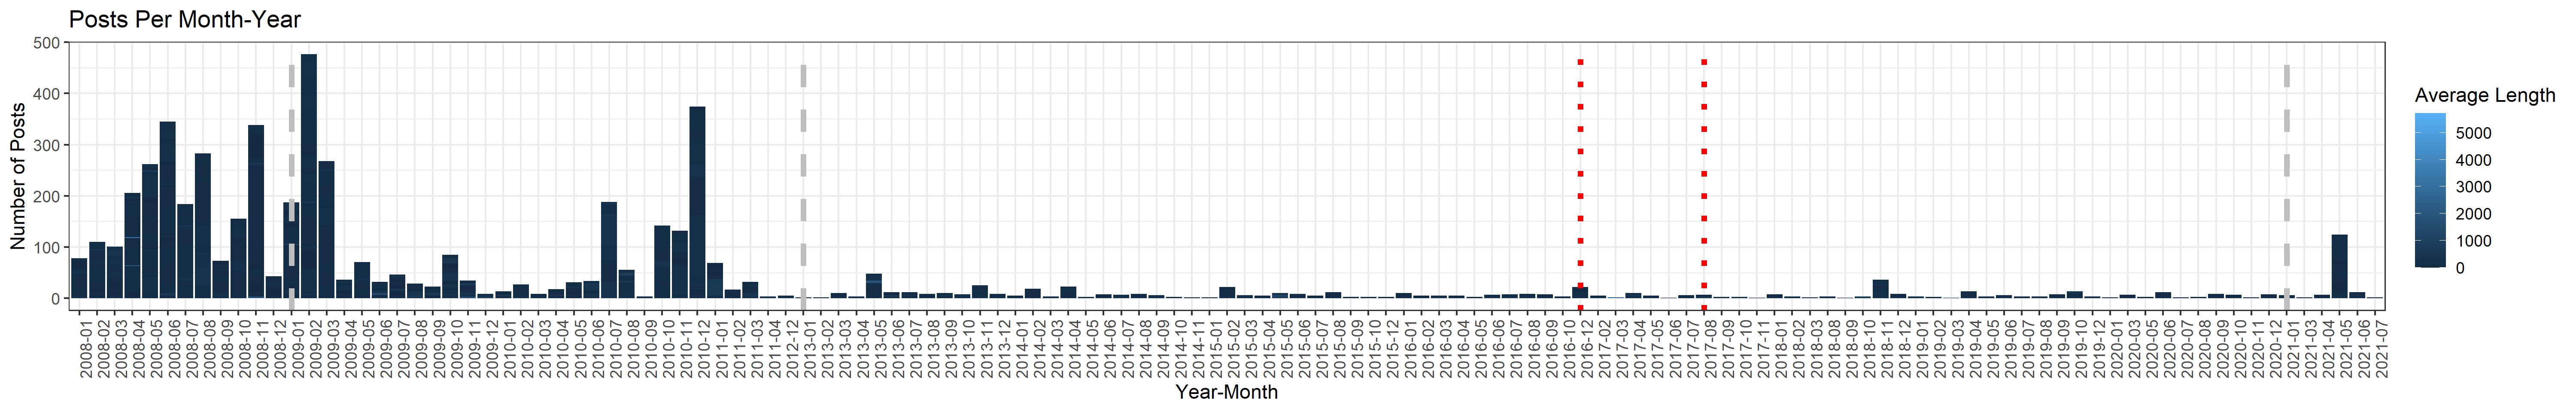
\includegraphics[width=.8\linewidth]{figs/ip_frequency_length.png}
	\caption{Post Prevalence and Length}
	\label{}
\end{figure}

Figure 1 shows post frequency on the forums over time. The majority of posts are under 1,000 words in length and forum activity spiked around the 2008 election of Barack Obama. It appears to be around this time (2008-2009) that private groups were created within the forum.

Given the somewhat-public facing nature of the forum, I predict that the general content of the forum will be \textit{positive} and community focused. Topic modeling should reveal the underlying content of the corpus and sentiment analysis should reveal generally positive, communal sentiment.

It must again be stressed that these predictions are intended to characterize only the corpus of forum posts presented here, not the tone and tambre of white nationalism in the United States. White nationalism and the white supremacist ideology behind it are unequivocally vitriolic and violent. However, I do not expect that rhetoric reflective of the violence undergirding this ideology will be prevalent on the public-facing side of the forum. With these data properly contextualized, and the understanding that any conclusions we draw from them represent how white nationalists want to present themselves to each other and anyone curious enough to trackdown their forum, I turn to my empirical analysis.

\section{Section II: Uncovering Post Topics}
There is a paucity of academic work utilizing StormFront.org posts to study white nationalists. The small body of relevant academic research has largely focused on developing models and algorithms for \textit{categorizing} StormFront.org content (CITE). This article, in contrast, introduces a method to automatically identify topics (not categories) within forum posts based only on the specific reports being analyzed. Topics represent latent structure in the corpus being analyzed. Relatively many topics will be present, to varying degrees, in any one forum post and many posts will include material about any one topic. The overall methodology does not rely on previously defined categories or training data and can be applied relatively rapidly by a single analyst.

I use structural topic modeling (STM) to uncover topics within the corpus of forum posts. STM is preferable to traditional Correlated Topic Models (CTM) and Latent Dirichlet Allocation (LDA) because STM allows topic prevalence and content to come from document metadata (CITE). In substantive terms, this means that I can avoid LDA’s more restrictive assumptions - in particular, the assumption that all inference can be drawn from the document text alone. Because I know my data concern various topics under the umbrella of white nationalism, but know \textit{a priori} that different forums may use different language to express the same sentiment within the context of the forum, methods like CTM and LDA are suboptimal. Structural topic modeling allows me to draw inferences based on post metadata - such as the forum to which it was posted.

\begin{figure} \centering
	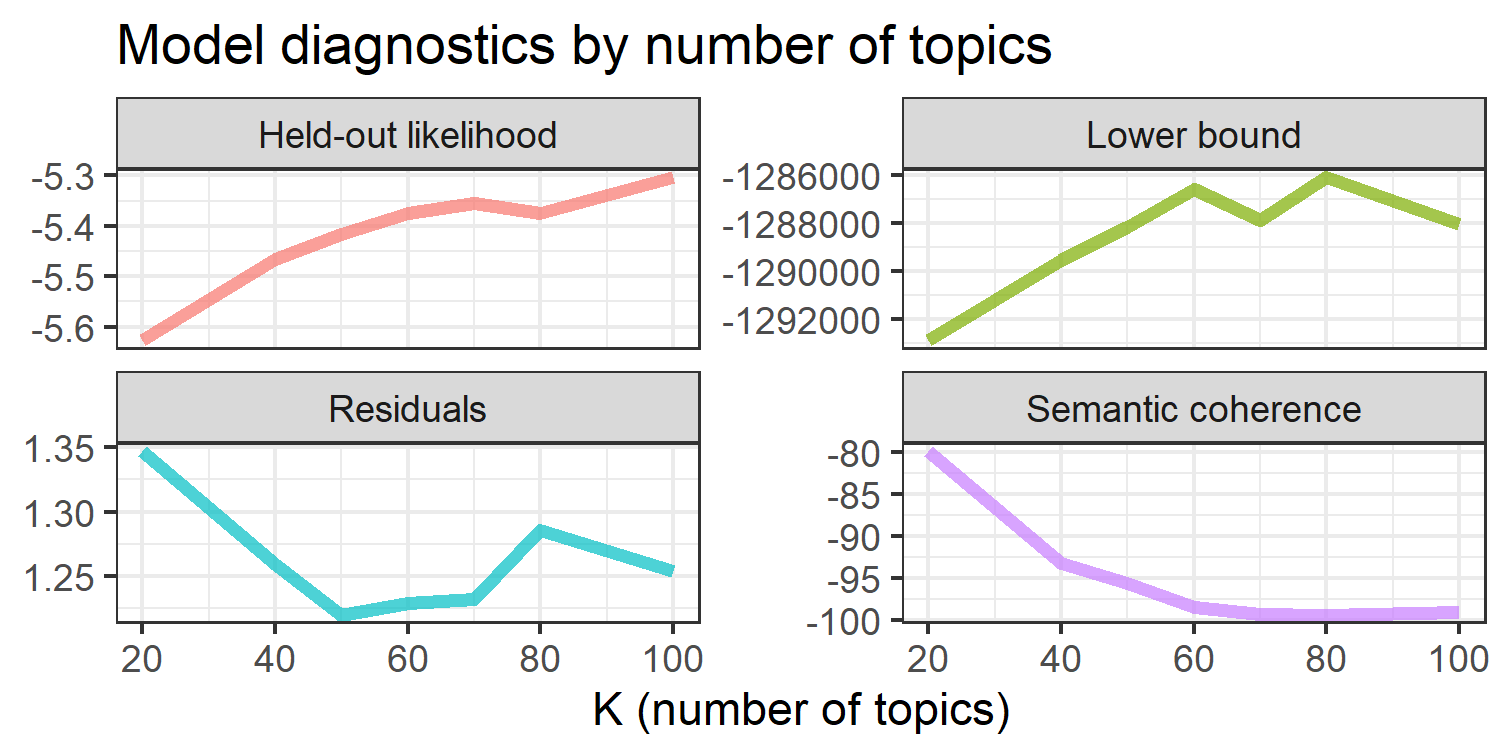
\includegraphics[width=.8\linewidth]{figs/diagnostics-by-topic.png}
	\caption{STM Results}
	\label{}
\end{figure}

I leverage the forum to which a text was posted to structure topic estimation. There is no way of knowing \textit{a priori} the appropriate number of topics to estimate, so I first estimated a series of 20, 50, 60, 80, and 100 topic models. The fit indices are shown in Figure 2. Ideally, the number of topics chosen will minimize the residuals and maximize the held-out likelihood. The basic idea of held-out likelihood is to hold out some fraction of the words in a set of documents, train the model and use the document-level latent variables to evaluate the probability of the held-out portion. By these metrics, a 60-70 topic model looks most appropriate. 

\begin{figure} \centering
	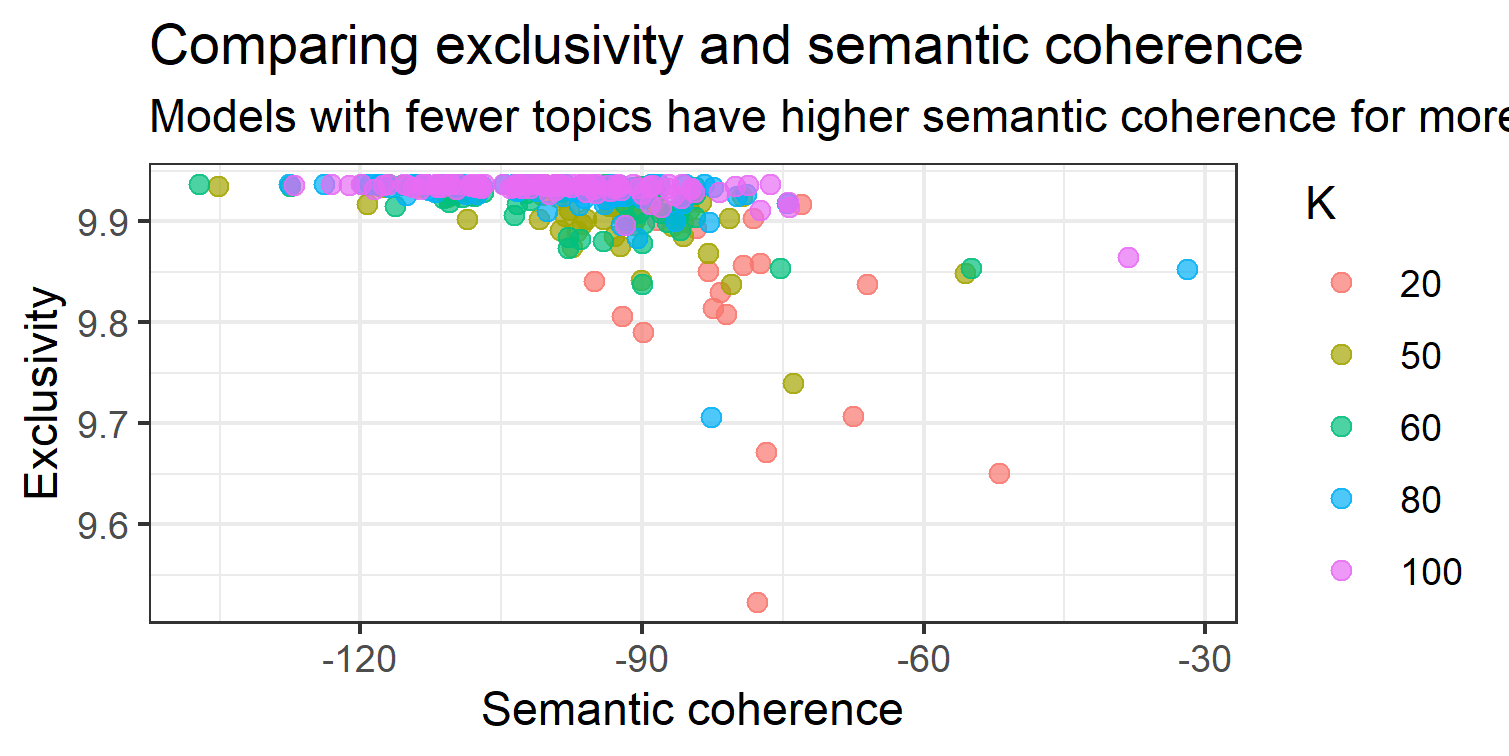
\includegraphics[width=.8\linewidth]{figs/exclusivity-vs-semantics.png}
	\caption{STM Results}
	\label{}
\end{figure}

However, ideally, we will also estimate a model high in both exclusivity and semantic coherence. Semantic coherence is high when the most probable words in a topic co-occur. Substantively, it maps on to topic quality and clarity. For example, we would expect ``Marx” and ``socialism” to co-occur in a well-fit model. Exclusivity captures the uniqueness of words to their topics. For example, it would be suboptimal if the word ``Marx” was a major contributing word to more than one topic because the more separate topics are from each other, the more we can learn from their presence/absence. There is a trade-off between semantic coherence and exclusivity.

\begin{figure} \centering
	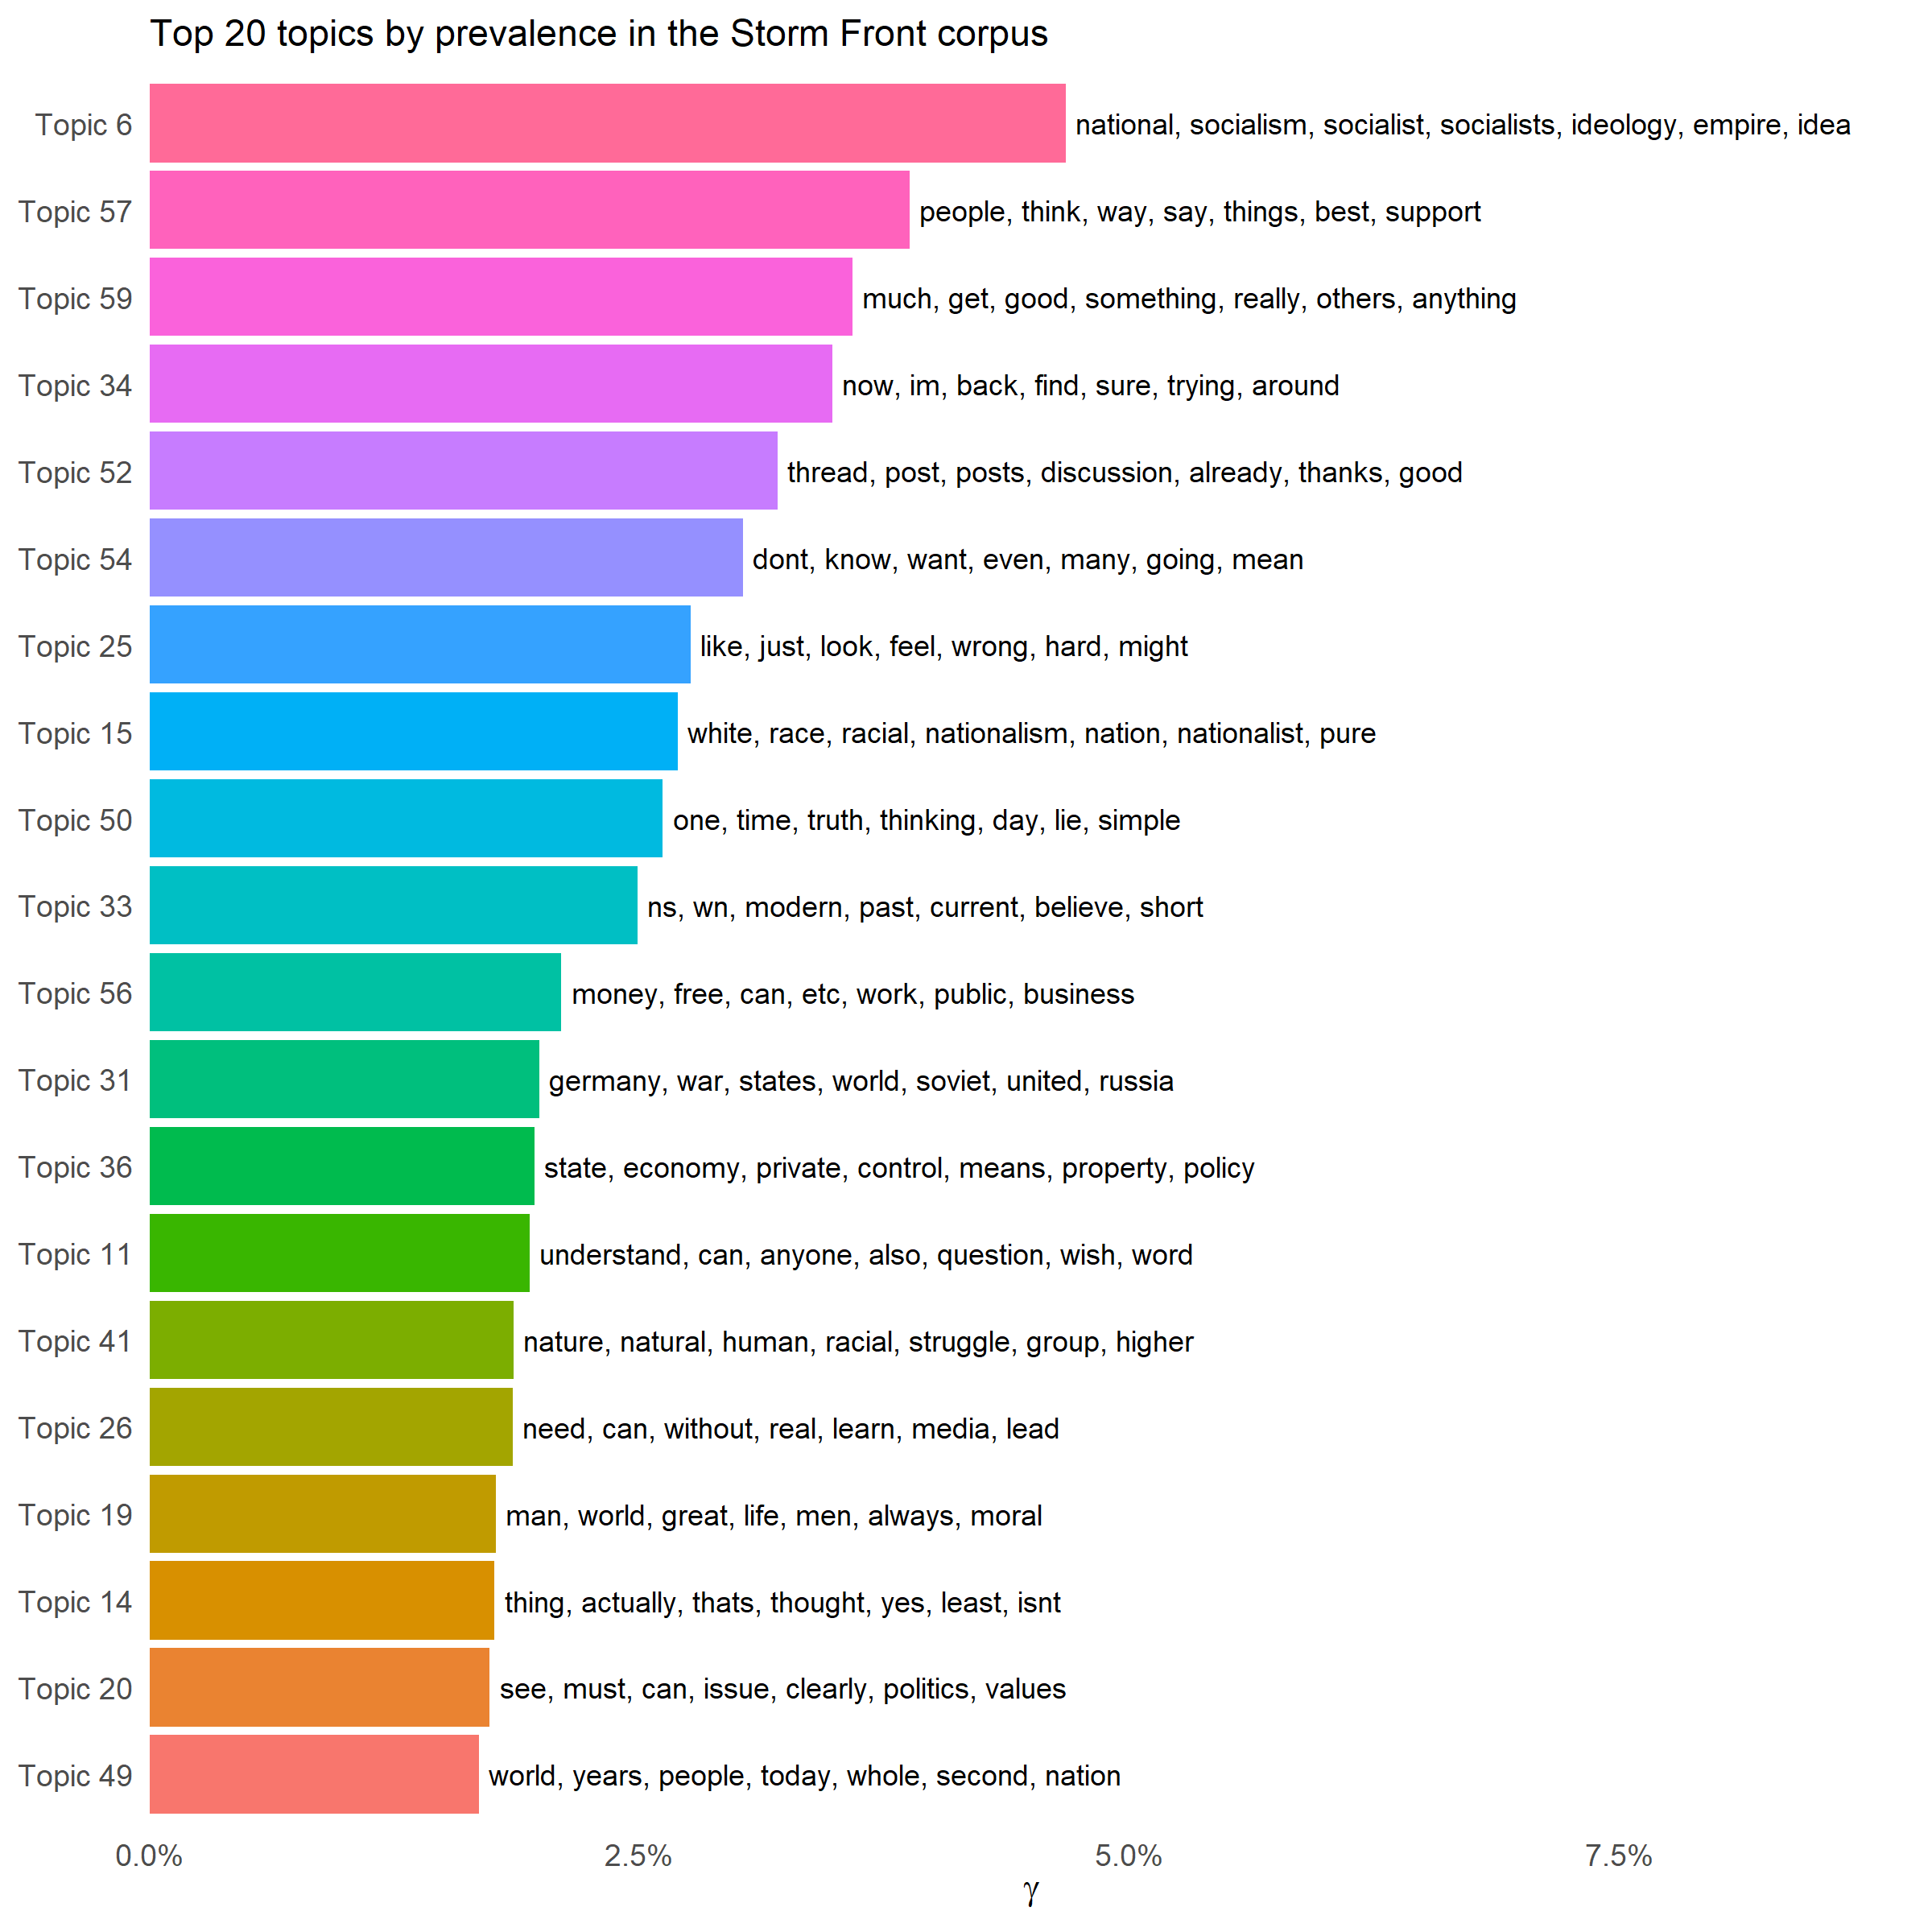
\includegraphics[width=.8\linewidth]{figs/top-20.png}
	\caption{STM Results}
	\label{}
\end{figure}

Given the clustering of estimates high in exclusivity and moderate in semantic coherence, I estimated a 60 topic model. The top 20 topics and the most prevalent words within those topics are shown in Figure 1 below, but a table with all 60 topics and prevalent words can be found in Appendix B.

As expected, given both the nature of StormFront.org and the Ideology and Philosophy subform, the most prevalent topic, Topic 6, is comprised of word-stems about nationalism, socialism, and ideology. Somewhat surprisingly, the next most-prevalent topic seems to focus on community; words like ``support" drive this topic. Language about race and white nationalism (wn) don't appear until the eighth most-prevalent topic.

To get a stronger idea of the sentiments contained within the corpus, I used the NRC Word-Emotion Association Lexicon (EmoLex) to uncover sentiment within the corpus (Mohammad and Turney 2010, 2013). The NRC EmoLex crowd-sourced the affective and emotional connotations of a variety of commonly-used words from native speakers. The results are striking and consistent with my prediction that the language used on StormFront.org will be quite positive. Indeed, the most frequently occurring sentiment is positivity.

\begin{figure} \centering
	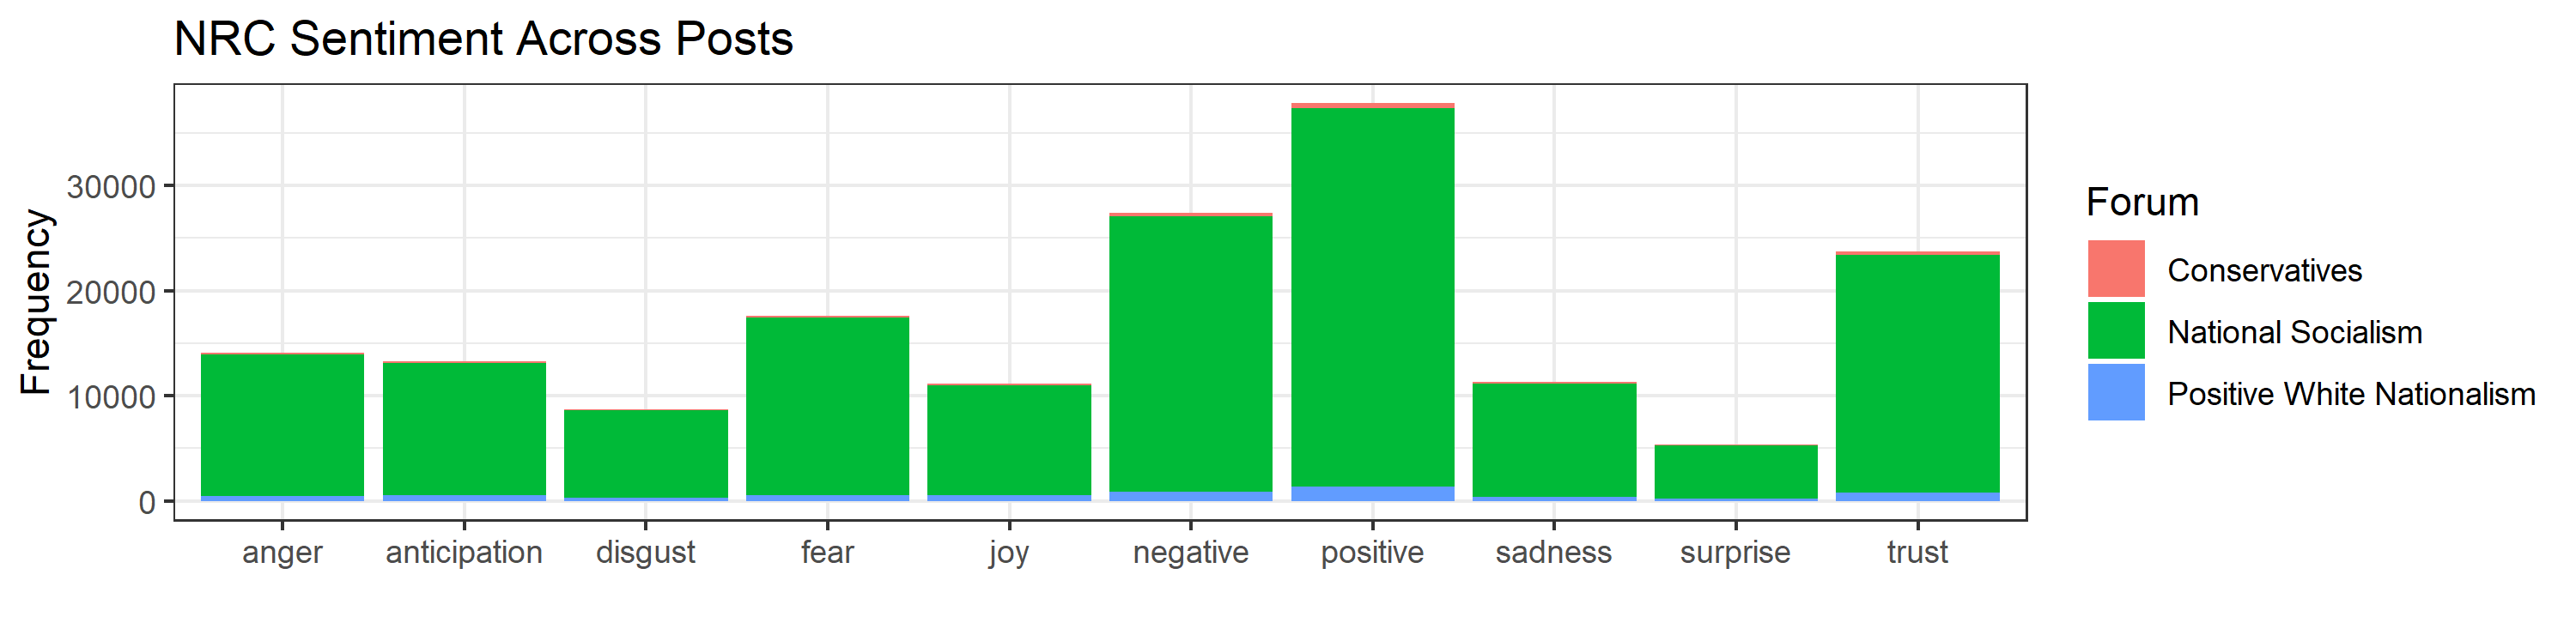
\includegraphics[width=.8\linewidth]{figs/sentiment_freq_all_words.png}
	\caption{NRC Sentiment Analysis}
	\label{}
\end{figure}

\section{Section III: Discussion}
To be written once I get past the initial shock of what's not visible on the public forum.









%%That table HERE
\begin{table}[H]
	\begin{adjustbox}{width=1\textwidth}
\begin{tabular}{lll}
	\multicolumn{1}{c}{\textbf{Topic}} & \multicolumn{1}{c}{\textbf{Expected Topic Proportion}} & \multicolumn{1}{c}{\textbf{Top 7 Terms}}                            \\
	Topic 6                            & 0.047                                                  & national, socialism, socialist, socialists, ideology, empire, idea  \\
	Topic 57                           & 0.039                                                  & people, think, way, say, things, best, support                      \\
	Topic 59                           & 0.036                                                  & much, get, good, something, really, others, anything                \\
	Topic 34                           & 0.035                                                  & now, im, back, find, sure, trying, around                           \\
	Topic 52                           & 0.032                                                  & thread, post, posts, discussion, already, thanks, good              \\
	Topic 54                           & 0.030                                                  & dont, know, want, even, many, going, mean                           \\
	Topic 25                           & 0.028                                                  & like, just, look, feel, wrong, hard, might                          \\
	Topic 15                           & 0.027                                                  & white, race, racial, nationalism, nation, nationalist, pure         \\
	Topic 50                           & 0.026                                                  & one, time, truth, thinking, day, lie, simple                        \\
	Topic 33                           & 0.025                                                  & ns, wn, modern, past, current, believe, short                       \\
	Topic 56                           & 0.021                                                  & money, free, can, etc, work, public, business                       \\
	Topic 31                           & 0.020                                                  & germany, war, states, world, soviet, united, russia                 \\
	Topic 36                           & 0.020                                                  & state, economy, private, control, means, property, policy           \\
	Topic 11                           & 0.019                                                  & understand, can, anyone, also, question, wish, word                 \\
	Topic 41                           & 0.019                                                  & nature, natural, human, racial, struggle, group, higher             \\
	Topic 26                           & 0.019                                                  & need, can, without, real, learn, media, lead                        \\
	Topic 19                           & 0.018                                                  & man, world, great, life, men, always, moral                         \\
	Topic 14                           & 0.018                                                  & thing, actually, thats, thought, yes, least, isnt                   \\
	Topic 20                           & 0.017                                                  & see, must, can, issue, clearly, politics, values                    \\
	Topic 49                           & 0.017                                                  & world, years, people, today, whole, second, nation                  \\
	Topic 2                            & 0.017                                                  & hitler, adolf, hitlers, speech, fact, later, made                   \\
	Topic 27                           & 0.016                                                  & us, let, believe, future, truly, enemies, come                      \\
	Topic 7                            & 0.016                                                  & point, however, seems, consider, different, believe, seem           \\
	Topic 58                           & 0.016                                                  & capitalism, communism, marxist, marx, marxism, fascism, class       \\
	Topic 45                           & 0.016                                                  & chapter, fight, existence, volume, hands, must, purity              \\
	Topic 37                           & 0.016                                                  & never, use, used, ive, seen, side, propaganda                       \\
	Topic 38                           & 0.015                                                  & party, political, nsdap, taken, program, organization, social       \\
	Topic 48                           & 0.015                                                  & new, old, revolution, republic, revolutionary, time, red            \\
	Topic 53                           & 0.015                                                  & aryan, european, culture, peoples, europe, blood, germanic          \\
	Topic 40                           & 0.015                                                  & well, said, die, put, done, re, saying                              \\
	Topic 22                           & 0.015                                                  & movement, ideas, term, call, cause, idea, views                     \\
	Topic 17                           & 0.014                                                  & american, america, history, black, americans, early, upon           \\
	Topic 46                           & 0.014                                                  & make, sense, makes, still, common, problems, fact                   \\
	Topic 47                           & 0.014                                                  & law, rights, right, must, state, demand, duty                       \\
	Topic 10                           & 0.014                                                  & nazi, nazis, nazism, communists, wasnt, nationalism, socialists     \\
	Topic 44                           & 0.014                                                  & power, form, freedom, democracy, political, leadership, rule        \\
	Topic 3                            & 0.013                                                  & first, better, two, comes, understanding, action, aware             \\
	Topic 23                           & 0.013                                                  & either, certain, terms, ie, much, rest, class                       \\
	Topic 12                           & 0.013                                                  & government, country, people, line, good, citizens, much             \\
	Topic 39                           & 0.013                                                  & course, perhaps, case, indeed, example, far, completely             \\
	Topic 4                            & 0.012                                                  & children, working, care, million, family, years, women              \\
	Topic 9                            & 0.012                                                  & whites, races, fight, taking, means, victory, nonwhites             \\
	Topic 21                           & 0.012                                                  & religion, christianity, christian, god, religious, speak, faith     \\
	Topic 13                           & 0.012                                                  & read, mein, book, reading, also, link, wrote                        \\
	Topic 42                           & 0.012                                                  & system, economic, capitalist, took, based, systems, view            \\
	Topic 51                           & 0.011                                                  & jews, jewish, jew, jesus, liberal, fact, lies                       \\
	Topic 55                           & 0.011                                                  & german, people, workers, germans, germany, international, destroyed \\
	Topic 5                            & 0.011                                                  & community, shall, within, purpose, society, individual, order       \\
	Topic 32                           & 0.011                                                  & another, points, tell, made, forum, ill, correct                    \\
	Topic 24                           & 0.010                                                  & kampf, original, interested, written, quotes, thoughts, mention     \\
	Topic 30                           & 0.010                                                  & true, right, left, stated, false, towards,                          \\
	Topic 8                            & 0.009                                                  & name, century, exactly, simply, came, matters, next                 \\
	Topic 28                           & 0.009                                                  & part, opinion, ideology, success, argument, death, greater          \\
	Topic 16                           & 0.009                                                  & every, person, quite, certainly, single, entire, fully              \\
	Topic 60                           & 0.009                                                  & place, long, become, fear, people, behind, even                     \\
	Topic 43                           & 0.009                                                  & last, reason, edited, pm, theres, real, made                        \\
	Topic 18                           & 0.008                                                  & go, found, enemy, spirit, words, civilization, western              \\
	Topic 29                           & 0.008                                                  & reich, third, history, german, youth, military, army                \\
	Topic 35                           & 0.006                                                  & agree, folk, der, im, folks, problem, nation                        \\
	Topic 1                            & 0.003                                                  & little, nietzsche, und, von, war, im, philosophy                   
\end{tabular}
\end{adjustbox}
\caption{Aid Programs by Type} 
\label{}
\end{table}









\end{document}